\documentclass[12pt,fleqn]{article}\usepackage{../common}
\begin{document}
Guven Araliklari, Hipotez Testleri

Guven Araliklari

Diyelim ki $X_1,..,X_i$ orneklemi birbirinden bagimsiz, ayni dagilimli ve
ortalamasi $\mu$, standart sapmasi $\sigma$ ve yine ayni olan bir nufus
dagilimindan geliyor. O zaman biliyoruz ki, Merkezi Limit Teorisi (Central
Limit Theorem) teorisine gore, orneklem ortalamasi $\bar{X} = \frac{1}{n}
X_1+..+X_n$, ortalamasi $\mu$, standart sapmasi $\sigma/n^2$ olan bir
normal dagilima yaklasiyor.

Peki veriyi (yani orneklemi) ve CLT'yi kullanarak $\mu$ hakkinda bir tahmin
yapabilir miyiz? Yani Buyuk Sayilar Kanunua gore $\mu$ hakkinda noktasal
tahmin yapabiliriz fakat, belki ondan bir adim otesi, bir ``guven araligi''
hesaplamaktan bahsediyoruz. Bu tahmin ``gercek $\mu$, \%95 ihtimalde su iki deger
arasindadir'' turunde bir tahmin olacak.

Bu araligin hesabi icin once $\bar{X}$'i standardize edelim, yani $N(0,1)$ haline cevirelim,

$$ Z = \frac{\bar{X} - \mu}{\sigma / \sqrt{n}} $$

Z-skorlarini isledigimiz yazida 

$$
P(z_1 < Z < z_2) =  \Phi(z_1) - \Phi(z_2) 
$$

gibi bir ifade gorduk. Esitligin sag tarafi aslinda bir alan hesabidir,
surekli fonksiyonlarda olasilik bir entegral, ya da iki kumulatif yogunluk
fonksiyonunun farki. Guven araligi icin bize lazim olan da bir olasilik,
hatta ``kesin'' bir olasilik, \%95 olasiligi. Demek ki esitligin sag tarafi
.95 olacak. .95 hesabi icin, normal egrisini dusunursek, sagindan ve
solundan 0.25 buyuklugunde iki parcayi ``kirpmamiz'' lazim. O zaman 0.975
olasiliginin z degeri ile, 0.025 olasiliginin z degeri arasindaki
olasilikta olmamiz lazim. Bu hesaplarda baz alinan $z_{\alpha/2}$ degeri ve
bu $100 \cdot \alpha / 2$ ust yuzdelik kismina, ornegimizde 0.975 kismina
tekabul ediyor. Normal dagilimin simetrisi sebebiyle onun eksisi alinmis
hali oteki (soldaki) parcayi verir, yani $-z_{\alpha/2}$. 

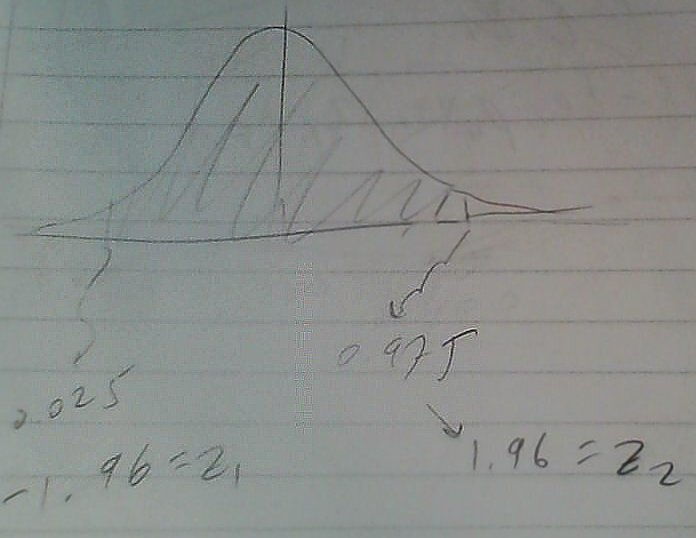
\includegraphics[height=6cm]{norm95.jpg}

Z-skoru hesaplarken tabloya danismistik, simdi tabloya tersinden bakacagiz,
kesisme noktasinda 0.975 diyen yeri bulup kordinatlari alacagiz, ki bu
deger 1.96. 

\begin{minted}[fontsize=\footnotesize]{python}
from scipy.stats.distributions import norm
print norm.ppf(0.975)
\end{minted}

\begin{verbatim}
1.95996398454
\end{verbatim}

Bazi Istatistik kaynaklarinda ``sihirli deger'' seklinde tarif edilen bir
deger bu, gozlerimiz kamasmasin, geldigi yer burasi iste. Simdi formulu
buna gore degistirelim,

$$ 
P \bigg( 
-z_{\alpha/2} \
\le \frac{\bar{X} - \mu}{\sigma / \sqrt{n}} 
\le z_{\alpha/2}
\bigg) = 1-\alpha
 $$

$P(\cdot)$ icinde biraz duzenleme, tum terimleri $\sigma / \sqrt{n}$ ile
carpalim, $\bar{X}$ cikartalim, ve $-1$ ile carpalim,

$$ 
P \bigg( 
\bar{X} - z_{\alpha/2}\frac{\sigma}{\sqrt{n}}
\le \mu
\le \bar{X} + z_{\alpha/2}\frac{\sigma}{\sqrt{n}}
\bigg) = 1-\alpha
 $$

Guven araligi ifadesine aslina erismis olduk. Eger \%95 kesinlikten
bahsediyor olsaydik, ve nufusun gercek varyansi $\sigma^2$ biliniyor
olsaydi, $P(\cdot)$ icine bu degerleri gececektik, $\bar{X}$ zaten verinin
aritmetik ortalamasindan ibarettir, bu bize $\mu$'nun solunda ve saginda
bazi degerler dondurecekti. Bu degerler bizim guven araligimiz
olacakti. Mesela veri 64.1, 64.7, 64.5, 64.6, 64.5, 64.3, 64.6, 64.8,
64.2, 64.3 seklinde, $n=10$ cunku 10 nokta var, $\sigma = 1$ olarak
verilmis.  Ortalamayi hesapliyoruz, 64.46. $\alpha=0.05$ icin

$$ 
P \bigg( 
64.46 - 1.96\frac{1}{\sqrt{10}}
\le \mu
\le 64.46 + 1.96\frac{1}{\sqrt{10}}
\bigg) = 0.95
 $$

$$ P\bigg(63.84 \le \mu \le 65.08\bigg) = 0.95 $$

Yani \%95 guven araligi $63.84 \le \mu \le 65.08$. 

Neler yaptik? CLT bilgisinden hareketle $\bar{X}$ hakkinda bir seyler
biliyorduk. Fakat $\bar{X}$'in {\em kesin} hangi normal dagilima
yaklastigini bilmek icin nufus paremetreleri $\mu,\sigma$ da
bilinmelidir. Diger yandan eger tek bilinmeyen $\mu$ ise, teoriyi bu
bilinmez etrafinda tamamen tekrar sekillendirip / degistirip CLT'yi
bilinmeyen $\mu$ etrafinda bir guven araligi yaratmak icin kullandik.

Kac Tane $n$?

Hatirlarsak guven araligini ustteki sekilde hesaplayabilmemizin sebebi CLT
sayesinde $\bar{X}$'in normal dagilima yaklasiyor olmasiydi. Ve, teoriyi
tekrar dusunursek yaklasma $n \to \infty$ oldugu zaman oluyordu. Buradan
$\bar{X}$'in normalliginin ``buyukce'' $n$ degerleri icin daha gecerli
olacagi sonucuna varabiliriz. Peki $n$ ne kadar buyuk olmali?  Literature
gore CLT'nin genellikle $n \ge 30$ durumunda gecerli oldugu soylenir. Tabii
nufus dagiliminin ne oldugu da onemlidir, eger nufus normal ise, ya da
genel olarak simetrik tek tepeli dagilim ise orneklem daha ufak kalsa da
bazi sonuclara varabiliriz. Eger nufus dagilimi cok yamuk (skewed),
etekleri genis dagilim ise o zaman daha buyuk orneklem daha iyi olur.

Soru

IO 800 yillarinda Italya'da Etrusali (Etruscan) toplumu vardi. Bu toplum
geldigi gibi birdenbire ortadan kayboldu. Bilimciler bu toplumun
Italyalilar ile fizyolojik, genetik ve kulturel olarak baglantisi olup
olmadigini hep merak etmistir. Bazilari hafa olculerine bakarak sonuclara
varmaya ugrasmistir. Arkeolojik kazilarda yapilan olcumlerde 84
Etrusyalinin kafasi olculmustur. Ayrica bugunku Italyanlarin kafa
olcumlerinin normal dagilimda $\mu=132.4 mm,\sigma=6.0mm$ oldugu
bilinmektedir. Iki toplum arasindaki baglanti kurmak icin, veriye bakarak
kafa olcumu ortalamasi icin bir \%95 guvenlik araligi olusturabiliriz, ve
eger bugunku Italyanlarin olcusu o araliga dusmuyorsa, Etrusyalilarla
baglantilarinin olmadigini iddia edebiliriz.

\begin{minted}[fontsize=\footnotesize]{python}
import pandas as pd
df = pd.read_csv('etrus.csv')
print float(df.mean()-1.96*(6.0/np.sqrt(84)))
print float(df.mean()+1.96*(6.0/np.sqrt(84)))
\end{minted}

\begin{verbatim}
142.524107721
145.09035011
\end{verbatim}

Bugunku Italyanlarin kafa ortalamasi $\mu=132.4$ bu araliga dusmuyor. Diger
bir deyisle, 84 tane orneklemden gelen orneklem ortalamasi 143.8 buyuk bir
ihtimalle $\mu=132.4,\sigma=6.0$ boyutlarindaki bir normal dagilimdan
gelmemistir. Buna gore, buyuk bir ihtimalle Etrusyalilar Italyanlarin atasi
degildir. 

Bilinmeyen $\sigma$

Guven Araliklari bolumunden devam edelim. Bilinmeyen $\mu$ durumunu
gorduk. Eger $\sigma$ bilinmiyorsa, bu durumda $\sigma$ yerine orneklem
varyansi $S$ kullanilabilir,

$$ S^2 = \frac{1}{n} \sum (X_i - \bar{X})^2
$$

ki ustteki degerin karekoku $S$ olacaktir. $\sigma$ yerine $S$ kullanmanin 
buyuk $n$ degerlerinde CLT'yi etkilemedigi ispat edilmistir [5]. 


Binom Dagilimlar ve Normal Yaklasiksallik

Binom ile Bernoulli dagilimi arasindaki baglantiyi biliyoruz. Diyelim ki
$X_1,..,X_n$ birbirinden bagimsiz ve ayni Bernoulli olarak dagilmis,
Bernoulli dagilimini temsil eden $Y$ tanimlayalim, o zaman

$$ Y = \sum_{i=1}^n X_i $$

Simdi orneklem ortalamasini hatirlayalim,

$$ \bar{X} = \frac{1}{n}  \sum_{i=1}^n X_i $$

O zaman 

$$ Y = n\bar{X}  $$

Merkezi Limit Teorisinden $\bar{X}$'in nufus beklentisi ve sapmasini iceren
$N(\mu,\sigma)$ olarak dagilacagini biliyoruz. Nufus parametreleri nedir?
Her $X_i$'in ayni olan $\mu,\sigma$'si ile alakli, durumda Bernoulli
parametrelerini alip $N(\cdot)$ icinde direk kullanabiliriz, 

$$E(X_i) = p, Var(X_i) = p(1-p)$$

o zaman 

$$\bar{X} \sim N(\mu,\sigma), \mu = p, \sigma = \sqrt{\frac{p(1-p)}{n}}$$

$Y$ ile $\bar{X}$ baglantisi: Bir genel teoriye gore eger $\bar{X}$ normal
ise $n\bar{X}$'in de normal oldugu bilinir, ve bu dagilim
$N(n\mu,\sqrt{n}\sigma)$ olarak gosterilir. Bu teorinin ispatini simdilik
vermeyecegiz. O zaman $Y = n\bar{X}$ is ve normal olarak dagilmis ise, o zaman 

$$ Y \sim N\bigg(np, \sqrt{np(1-p)}\bigg)$$

demek dogru olacaktir. Standardize etmek gayet basit,


$$Z  = \frac{Y - np}{\sqrt{np(1-p)}}$$

ya da, bolum ve boleni $n$ ile bolersek,

$$Z  = \frac{Y/n - p}{\sqrt{p(1-p)/n}}$$


$$Z  = \frac{Y/n - p}{\sqrt{\frac{p(1-p)}{n}}}$$

Soru

Amerikalilarin yuzde 12'sinin zenci oldugunu biliyoruz. Eger 1500 kisiyi
iceren bir orneklem alsaydik, bu orneklemde 170'den daha az zenci
olmasinin olasiligi nedir? 

Cevap

\%12 nufus parametresidir, yani $p=0.12$. Orneklem $n=1500$. Normal
yaklasiksallamasi ile 

\begin{minted}[fontsize=\footnotesize]{python}
from scipy.stats import norm
n = 1500
p = 0.12
mu = n*p
std = np.sqrt(n*p*(1-p))
print mu,std
print 'olasilik',norm.cdf(170,loc=mu,scale=std)
\end{minted}

\begin{verbatim}
180.0 12.585706178
olasilik 0.213437028747
\end{verbatim}

Yani $N(180,12.58)$ dagilimini elde ettik ve hesaplari onun uzerinden
yaptik. Sonuc diyor ki verilen orneklem ve nufus $p$ degeri ile 170 altinda
zenci sayisi elde etmek oldukca dusuk bir ihtimalde. 

Ornek

Diyelim ki elimizde bir Web sitesinin gunluk ziyaret, tiklama sayilarini
gosteren bir veri seti var, CVR ziyaretcilerin sitedeki tiklayan musteriye
donusmesi orani (conversion). 

\begin{minted}[fontsize=\footnotesize]{python}
import pandas as pd
from scipy import stats
a = pd.DataFrame({'tiklama': [20.,2.,40.,5.,10.,100.],
                  'ziyaret': [100.,10.,300.,400.,30.,800.]})
a['cvr'] = a['tiklama'] / a['ziyaret'] 
print a
\end{minted}

\begin{verbatim}
   tiklama  ziyaret       cvr
0       20      100  0.200000
1        2       10  0.200000
2       40      300  0.133333
3        5      400  0.012500
4       10       30  0.333333
5      100      800  0.125000
\end{verbatim}

Bu veri seti icin cvr'in 0.16, yani yuzde 16 oldugunu onceden
biliyoruz. Ustteki basari orani binom dagili ile modellenebilir, ziyaretler
"deneylerdir", yani orneklem buyuklugunu gosterirler. Tiklama ise
basaridir, onceki binom ornegindeki ayni formulu kullanirsak, normal
yaklasiksalligi uzerinden bir z-skoru hesaplayabiliriz,

\begin{minted}[fontsize=\footnotesize]{python}
p = 0.16
btest = lambda x: (x['cvr']-p) / np.sqrt( p*(1-p)/x['ziyaret'])
a['guven'] = a.apply(btest, axis=1)
a['guven'] = np.round(stats.zprob(a['guven'])*100,2)
print a
\end{minted}

\begin{verbatim}
   tiklama  ziyaret       cvr  guven
0       20      100  0.200000  86.24
1        2       10  0.200000  63.50
2       40      300  0.133333  10.39
3        5      400  0.012500   0.00
4       10       30  0.333333  99.52
5      100      800  0.125000   0.35
\end{verbatim}

Binom Guven Araligi

Binom'un Normal yaklasiksalligi konusundan bir ornek daha. Eger $p$
bilinmiyor ise onun icin maksimum olurluk tahmin edicisi (maximum
likelihood estimator) $Y/n$'dir. Ispat icin ek bolumune bakabiliriz.

$$Z  = \frac{X/n - p}{\sqrt{\frac{(X/n)(1-(X/n))}{n}}}$$

Ustteki ifade yaklasiklalliktan geliyor. Bu durumda $Z$ uzerinden, aynen
daha once yaptigimiz gibi, bir guvenlik araligi tanimlayabiliriz. 

$$ 
P \bigg( 
-z_{\alpha/s} \le
\frac{X/n - p}{\sqrt{\frac{(X/n)(1-(X/n))}{n}}} \le 
z_{\alpha/s}
\bigg) =
1-\alpha
$$

ve yine daha oncekine benzer cebirsel islemler sonrasi, ve Binom deneydeki
basari sayisi olarak $X$ yerine $k$ kullanalim, $P()$ ifadesini cikartalim,
cunku zaten o ifadenin icinde olusacak sayilarla ilgileniyoruz,

$$ 
\bigg( 
\frac{k}{n}-
z_{\alpha/s}\sqrt{\frac{(k/n)(1-(k/n))}{n}}
,
\frac{k}{n} +
z_{\alpha/s} \sqrt{\frac{(k/n)(1-(k/n))}{n}}
\bigg)
$$

Ustteki iki sayi bize gerekli guven araligini verecektir. 

Soru 

Amerika'da 2009 yilinda halkin ne kadarinin arabalarinda yakit tasarrunu
destekledigi merak konusuydu. Bir Gallup telefon anketinde bu soru 1012
yetiskine (18 ve ustu yasta) soruldu. Cevap 810 kisinin tasarrufu
destekledigi yonundeydi. Yani $n=1012,k=810$. O zaman $p$ icin \%95 guven
araligini bulun.

Cevap 

$$ \bigg(
\frac{810}{1012}-1.96 \frac{(810/1012)(1-810/1012)}{1012} ,
1.96 \frac{(810/1012)(1-810/1012)}{1012}
\bigg)
$$

$$ = (0.776,0825) $$


Hata Payi (Margin of Error)

Basinda oranlari rapor ederken onunla beraber telafuz edilen bir kavram
hata payidir. Aslinda bu binom dagilimlarda guven araligi ile cok yakinda
alakalidir;  hata payi \%95 guven araliginin en maksimum genisliginin yarisi
olarak bilinir. Yani \%95 araliginin bir ucunu diger ucundan cikartirsak ve
ikiye bolersek, istenen sonuca erisiriz. Formulsel olarak genislik $w$,

$$ w = \frac{k}{n} + 
1.96 \sqrt{\frac{(k/n)(1-k/n)}{n}} - 
- \bigg[ 
\frac{k}{n} -
1.96 \sqrt{\frac{(k/n)(1-k/n)}{n}}
\bigg]
 $$

$$ = 3.92 \sqrt{\frac{(k/n)(1-k/n)}{n}} $$

Simdi $(k/n)(1-k/n)$ carpimini dusunelim. {\em Orneklem Buyuklugu}
bolumunde gorduk, $n$ her zaman $k$'den buyuk olduguna gore $k/n$ her zaman
0 ve 1 arasindadir, o zaman $(k/n)(1-k/n) \le 1/4$ olmalidir, yani
gosterilen carpim 1/4'ten buyuk olamaz. Bunu alip ustteki formul icine
koyarsak,

$$ \max w = 3.92 \sqrt{\frac{1}{4n}} $$

elde ederiz. Bunun yarisi hata payidir $d$ olur, yani

$$ d = \frac{0.98}{\sqrt{n}} $$

Ornek

Bir secim kampaynasi sirasinda A ve B adaylari arasinda hangisinin daha
once oldugunu bulmak icin bir anket yapilir. Telefonda 597 kisiye
soruldugunda A adayinin 299 kisinin oyunu alacagi saptanmistir. Basin
durumu ``A adayinin avantaji hata payi \%4 icinde oldugu icin o onde kabul
edilebilir'' diye rapor etmistir. A oylarinin hata payi hakikaten \%4'mudur?

\begin{minted}[fontsize=\footnotesize]{python}
n = 597.
k = 299
print n/2
print k/n
d = 0.98/np.sqrt(n) 
print d*100
\end{minted}

\begin{verbatim}
298.5
0.500837520938
4.01087299444
\end{verbatim}

Evet hata payi \%4 cikti. 

Dikkat edilirse hata payinin anketten gelen sonuclarla hicbir alakasi yok,
A icin tercih \%25, \%75 olabilirdi ama ustteki hata payi hesabi yine ayni
kalirdi. Bunun sebebi formulun $n$'ye bagli olmasi. 

Daha onemli soru hata payi basinin ustteki ifadesinin gercekten secim
sonucu ile alakali olup olmadigi! 

Hipotez Testleri (Hypothesis Testing)

Istatistik tek ya da araliklar olarak sayisal tahminler uretmenin otesinde,
``iki sey arasinda birisini secmek'' turunde bir karar baglaminda da
kullanilabilir. Bir psikolog bir davaya uzman gorus vermek icin
cagrilmistir ve sanik hakkinda 'akli olarak dengesiz ya da dengeli'
arasinda bir secim yapacaktir. Ilac regulasyonu ile ugrasan kurum yeni bir
ilac hakkinda 'etkili' ya da 'etkisiz' seklinde bir karara ulasacaktir. 

Bir deneyin mumkun sonuclarini belli seceneklere yonlendirip olasilik
teorisini kullanarak bunlardan birisini secmeye Istatistik biliminde
Hipotez Test Etmek adi verilir.  

Birbiriyle yaris halinde olan iki hipotez vardir, bunlar sifir hipotezi
($H_0$ olarak yaziliyor) ve alternatif hipotezdir ($H_1$ olarak
yaziliyor). $H_o$ ve $H_1$ arasinda nasil secim yapacagimiz kavramsal
olarak bir davada jurinin yaptigi secime benzer: aynen sanigin, tersi
ispatlanana kadar, masum kabul edilmesi gibi eger veri tersi sonuca varmaya
yetmezse $H_0$ da ``kabul edilir'', yani sucsuzlugun devam etmesi gibi
$H_0$ gorusu terkedilmemis olur. Statusko devam eder. Bu karari verirken
mahkemenin kanitlari incelemesi, hipotez testinde rasgele degiskenlerle
verinin uzerinden hesaplar yapmaya benzer.

Bunu bir ornek uzerinden daha iyi anlayabiliriz. Diyelim ki araba ureten
bir sirket yakit performansini (gas mileage) arttirmaya ugrasiyor. Benzine
katilan yeni bir madde uzerinde deneyler yapiyorlar, deney icin Boston /
Los Angeles arasinda 30 tane araba sefer yapiyor. Yeni katki maddesi
olmadigi durumda (statuko) yakit performansinin ortalama 25.0 mil/galon ve
standart sapmanin 2.4 mil/galon oldugu biliniyor. Diyelim ki deney
sonrasinda arabalar ortalama olarak $\bar{y}$=26.3 mil/galon performansi
gostermisler. Katki maddesi etkili mi, etkili degil mi?

Arastirmacilar 25.0'dan 26.3'e olan degisikligi daha once bahsettigimiz
mahkeme ornegindeki gibi bir cercevede incelerler. Tipik olarak sifir
hipotezi statukoyu temsil eder, yani degismesi icin ``ezici sekilde aksi
yonde veri olmasi gereken sey'' budur. Oyle degil mi? Eger etkisiz bir
katki maddesine evet dersek, ve ileride oyle olmadigi belli olursa bunun
sirket icin cok negatif etkileri olacaktir, aynen masum bir kisiyi
yanlislikla hapse atmis olmak gibi. O yuzden kalmak istedigimiz guvenli
konum $H_0$'i temsil etmelidir. 

Bu noktada problemi rasgele degiskenlerin terminolojisi uzerinden tekrar
tanimlamak faydali olur. Diyelim ki test sirasinda 30 tane aldigimiz olcum
$y_1,..,y_n$, her $y_i$ normal olarak dagilmis ve bu dagilimlarin $\mu$'su
ayni, ve $\mu$'u birazdan ``eski'' olcumlerin ortalamasi olarak alacagiz,
cunku curutmek istedigimiz hipotez bu. Ayrica daha onceki tecrubelerimiz
gosteriyor ki $\sigma = 2.4$. Yani,

$$ 
f_Y(y;\mu) = \frac{1}{\sqrt{2\pi}(2.4)} 
e^{-\frac{1}{2}(\frac{y-\mu}{2.4})^2},
-\infty < y < \infty
$$


Hipotezleri soyle tanimlayalim,

$H_0$: $\mu = 25.0$ (Katki maddesi etkili {\em degildir})

$H_0$: $\mu > 25.0$ (Katki maddesi etkilidir)

Simdi yeni dagilimi standardize edip, bir hayali ortalama esik degeri
uzerinden bir sonuc cikartalim, standardize etmek icin kullandigimiz $\mu =
25.0$
cunku eski ortalama bu. Simdi diyelim ki test ettigimiz esik deger 25.25
(esas  amac 26.3 ama oraya gelecegiz), aradigimiz olasilik,

$$ P(\bar{Y}  \ge 25.25) $$

Ustteki ifade ``eger orneklem eski dagilimdan geliyor olsaydi, 25.25
esik degerini gecmesi ne kadar mumkun olabilirdi'' diye bir soru
soruyor. $\bar{Y}$'yi standardize edelim, o sirada esitsizligin sag tarafi da
degisir,

$$ P(\frac{\bar{Y} - 25.0}{2.4 / \sqrt{30}} \ge 
\frac{25.25 - 25.0}{2.4 / \sqrt{30}}) 
$$


$$ P(Z \ge 0.57)$$

z-Skoru tablosunu kullanakarak bu hesabi yapmak icin

$$ 1 - P(Z < 0.57)$$

0.57'nin z-skoru (satir 0.5 kolon .07) 0.7157 olarak gosterilmis, o zaman
1-0.7157 = 0.2843. Kod ile

\begin{minted}[fontsize=\footnotesize]{python}
print 1-norm.cdf(0.57)
\end{minted}

\begin{verbatim}
0.284338849046
\end{verbatim}

Demek ki

$$ P(Z \ge 0.57) = 0.2843$$

Demek ki yeni deney sonuclarinin, eski dagilima gore, esik degerinden fazla
gelmesi hala az da muhtemel, demek ki eski hipotezi tam
curutemedik. Sectigimiz esik degeri bize kesin bir sonuc saglamadi,
sezgisel olarak bu olasiligin buyuk oldugunu goruyoruz. Mahkeme durumunda
sucsuz olmasi cok muhtemeldir diyemiyoruz. Ya da araba orneginde (ve
pozitif baglamda) yeni yakit kesinlikle farklidir / fazladir
diyemiyoruz. Bize daha kesin noktalar lazim, aklimizda bize ``acaba?''
dedittirecek esik degerler istemiyoruz.

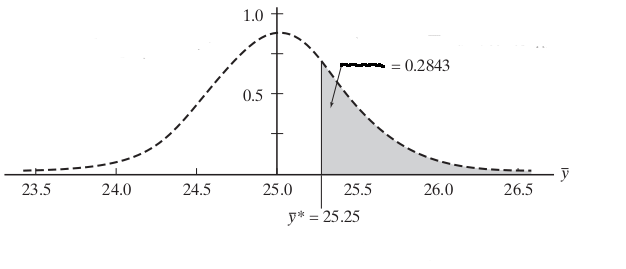
\includegraphics[height=6cm]{carhyp1.png}

Hayali esik noktasi $\bar{y}^*$'nin daha buyuk yapsak (ki o zaman ona bagli
olan sagdaki olasilik kuculecek). Bu olur mu? Eger $\bar{y}^* = 26.50$
olsaydi? 

$$ P(\frac{\bar{Y} - 25.0}{2.4 / \sqrt{30}} \ge 
\frac{26.50 - 25.0}{2.4 / \sqrt{30}}) 
$$

$$ P(Z \ge 3.42) $$

$$ = 0.0003 $$

Bu olasilik ise cok kucuk, yani esik degeri cok buyuk! Citayi cok fazla
kaldirdik, mahkeme durumunda sanki diyoruz ki sucun 1000 tane tanigi lazim,
sanik sucunu itiraf etmis olmali, hersey apacik olmali, bir de herseyi
bizzat ben gormus olmaliyim, yoksa kabul etmem. Araba orneginde katki
maddesi arabaya Formula-1 yarisi kazandirmazsa biz bu yakiti daha iyi
olarak kabul etmeyiz diyoruz.

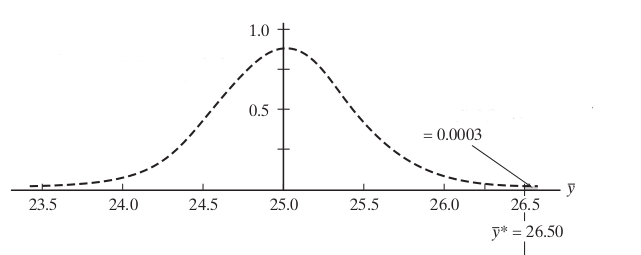
\includegraphics[height=6cm]{carhyp2.png}

Peki eger 0.28 cok fazla, 0.0003 cok kucuk ise hangi olasilik en iyi esik
degerini verir? Bu soruya kesin olarak ve matematiksel bir cevap vermek
mumkun degil, fakat hipotez test etme teknigini kullanan arastirmacilarin
ulastigi konsensus 0.05 olasilik seviyesinin en iyi sonuclar verdigidir. Bu
duruma sifir hipotezinin cok kolayca kenara atilmamasi, ya da ona
gereginden fazla bagli kalinmamasi mumkun oluyor.

O zaman 0.05 olasiligini verdirtecek esik degeri hesaplayalim,

$$ P(\frac{\bar{Y} - 25.0}{2.4 / \sqrt{30}} \ge 
\frac{\bar{y}^* - 25.0}{2.4 / \sqrt{30}}) = 0.05
$$

$$ P(Z \ge  \frac{\bar{y}^* - 25.0}{2.4 / \sqrt{30}}) = 0.05
$$
ya da

$$ P(Z \le  \frac{\bar{y}^* - 25.0}{2.4 / \sqrt{30}}) = 0.95 $$

z-Skor tablosuna bakiyoruz, ``hangi z degeri 0.95 degeri sonucunu verir'',
kordinatlardan 1.64 z-skorunu buluyoruz. Ya da

\begin{minted}[fontsize=\footnotesize]{python}
print norm.ppf(0.95)
\end{minted}

\begin{verbatim}
1.64485362695
\end{verbatim}


$$ P(Z \le 1.64)  = 0.95 $$
O zaman 

$$ \frac{\bar{y}^* - 25.0}{2.4 / \sqrt{30}} = 1.64 $$

ve buradan $\bar{y}^* = 25.178$ sonucu cikiyor. 26.3 degeri bu degerden
yuksektir demek ki sifir hipotezi curutulmustur. Yeni yakit katkisinin
performansi arttiriyor olmasi buyuk bir olasiliktir. 

Not: Bu testi aslinda daha basit sekilde $\bar{y}^* = 26.3$ degerlerini
vererek elde edilen degeri 0.05'ten kucuk olup olmadigina bakarak ta
yapabilirdik. Fakat metotu insa ediyorduk o sebeple daha fazla ornekli
anlatmak gerekti. 

Ornek

SAT-I testinde ulke averajina oldukca yakin sonuclar alan bir lisede yeni
bir mufredat denenmesine karar veriliyor. Deneme icin 86 ogrenci rasgele
sekilde seciliyor ve yeni bir tur cebir ve geometri dersine
sokuluyor. Sonraki SAT-1 testinde sonuclarina gore bu cocuklar ortalama 502
sonuc almislar, ulke capindaki ortalama 494, standart sapma
124. $\alpha=0.05$ onemliligi (significance) seviyesinde yeni mufredatin
basarili oldugu iddia edilebilir mi? 

Ilk once $\mu$ parametresinin yeni mufredatin gercek ortalamasi oldugunu
farzediyoruz. O zaman statusko nedir? Bu ortalamanin ulke ortalamasi
seviyesinde kalmasidir, yani $\mu_0 = 494$ olmasidir. Fakat bu sefer
alternatif hipotez iki yonlu (two-sided) olmali cunku yeni mufredat hic
istenmese de test sonuclarinda negatif sonuca da yol acabilir! O zaman
$H_0$'i reddetmeliyiz eger z istatistigi $\le -z_{0.025}$ ise (yani
-1.96'dan kucuk ise), ya da $\ge z_{0.025}$ (yani 1.96'dan buyuk ise). 

$$ z = \frac{502-494}{124\sqrt{86}} = 0.60$$

Sonuc 1.96'dan buyuk degil. O zaman $H_0$'i, yani statukoyu
degistiremedik. Elde edilen sonuclar bir ilerlemedir fakat bu ilerlemenin sans
eseri olmasi da muhtemel.

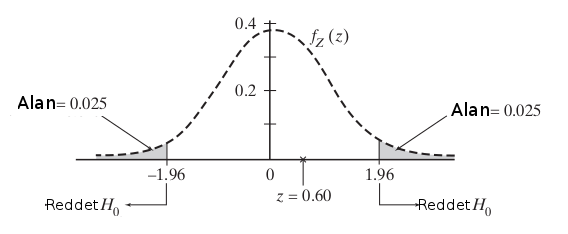
\includegraphics[height=5cm]{sat1.png}

Tek Orneklem t Testi (One-sample t test)

Bu test verinin Normal dagilimdan geldigini farzeder, tek orneklem
durumunda elde $x_1,...,x_n$ verisi vardir, ve bu veri $N(\mu,\Sigma)$
dagilimindan gelmistir ve test etmek istedigimiz hipotez /
karsilastirma $\mu = \mu_0$. 

\begin{minted}[fontsize=\footnotesize]{python}
from scipy.stats import ttest_1samp, wilcoxon, ttest_ind
import pandas as pd
daily_intake = np.array([5260,5470,5640,6180,6390,6515, 6805,7515,7515,8230,8770])
df = pd.DataFrame(daily_intake)
print df.describe()
\end{minted}

\begin{verbatim}
                 0
count    11.000000
mean   6753.636364
std    1142.123222
min    5260.000000
25%    5910.000000
50%    6515.000000
75%    7515.000000
max    8770.000000
\end{verbatim}

\begin{minted}[fontsize=\footnotesize]{python}
t_statistic, p_value = ttest_1samp(daily_intake, 7725)
print "one-sample t-test", p_value
\end{minted}

\begin{verbatim}
one-sample t-test 0.0181372351761
\end{verbatim}

Sonuc \verb!p_value! \verb!0.05!'ten kucuk cikti yani
yuzde 5 onemliligini (significance) baz aldik bu durumda veri
hipotezden onemli derecede (significantly) uzakta. Demek ki
ortalamanin 7725 oldugu hipotezini reddetmemiz gerekiyor.

Testi iki orneklemli kullanalim, gruplar 0/1 degerleri ile
isaretlendi, ve test etmek istedigimiz iki grubun ortalamasinin (mean)
ayni oldugu hipotezini test etmek. t-test bu arada varyansin ayni
oldugunu farzeder.

\begin{minted}[fontsize=\footnotesize]{python}
energ = np.array([
[9.21, 0],
[7.53, 1],
[7.48, 1],
[8.08, 1],
[8.09, 1],
[10.15, 1],
[8.40, 1],
[10.88, 1],
[6.13, 1],
[7.90, 1],
[11.51, 0],
[12.79, 0],
[7.05, 1],
[11.85, 0],
[9.97, 0],
[7.48, 1],
[8.79, 0],
[9.69, 0],
[9.68, 0],
[7.58, 1],
[9.19, 0],
[8.11, 1]])
group1 = energ[energ[:, 1] == 0][:, 0]
group2 = energ[energ[:, 1] == 1][:, 0]
t_statistic, p_value = ttest_ind(group1, group2)
print "two-sample t-test", p_value
\end{minted}

\begin{verbatim}
two-sample t-test 0.00079899821117
\end{verbatim}

$p-value < 0.05$ yani iki grubun ortalamasi ayni degildir. Ayni oldugu
hipotezi reddedildi.

Eslemeli t-Test (Paired t-test)

Eslemeli testler ayni deneysel birimin olcumu alindigi zaman
kullanilabilir, yani olcum alinan ayni grupta, deney sonrasi deneyin
etki edip etmedigi test edilebilir. Bunun icin ayni olcum deney
sonrasi bir daha alinir ve "farklarin ortalamasinin sifir oldugu"
hipotezi test edilebilir. Altta bir grup hastanin deney oncesi ve
sonrasi ne kadar yiyecek tukettigi listelenmis. 

\begin{minted}[fontsize=\footnotesize]{python}
intake = np.array([
[5260, 3910],
[5470, 4220],
[5640, 3885],
[6180, 5160],
[6390, 5645],
[6515, 4680],
[6805, 5265],
[7515, 5975],
[7515, 6790],
[8230, 6900],
[8770, 7335],
])
pre = intake[:, 0]
post = intake[:, 1]
t_statistic, p_value = ttest_1samp(post - pre, 0)
print "paired t-test", p_value
\end{minted}

\begin{verbatim}
paired t-test 3.05902094293e-07
\end{verbatim}

Wilcoxon isaretli-sirali testi (Wilcoxon signed-rank test)

t Testleri Normal dagilima gore sapmalari yakalamak acisindan,
ozellikle buyuk orneklemler var ise, oldukca saglamdir. Fakat bazen
verinin Normal dagilimdan geldigi faraziyesini yapmak istemeyebiliriz.
Bu durumda {\em dagilimdan bagimsiz metotlar} daha uygundur, bu tur
metotlar icin verinin yerine cogunlukla onun sira istatistiklerini
(order statistics) kullanir.

Tek orneklemli Wilcoxon testi icin prosedur $\mu_0$'i tum veriden
cikartmak ve geri kalan (farklari) isaretine bakmadan numerik degerine
gore siralamak, ve bu sira degerini bir kenara yazmak. Daha sonra geri
donup bu sefer cikartma islemi sonucunun isaretine bakmak, ve eksi
isareti tasiyan sira degerlerini toplamak, ayni islemi arti isareti
icin yapmak, ve eksi toplami arti toplamindan cikartmak. Sonucta
elimize bir istatistik $W$ gelecek. Bu test istatistigi aslinda $1..n$
tane sayi icinden herhangi birini $1/2$ olasiligiyla secmek, ve
sonuclari toplamaya tekabul etmektedir. Ve bu sonuc yine \verb!0.05!
ile karsilastirilir.

\begin{minted}[fontsize=\footnotesize]{python}
z_statistic, p_value = wilcoxon(daily_intake - 7725)
print "one-sample wilcoxon-test", p_value
\end{minted}

\begin{verbatim}
one-sample wilcoxon-test 0.0279991628713
\end{verbatim}

Hipotezi yine reddettik.

Ustte yaptigimiz eslemeli t-testi simdi Wilcoxon testi ile yapalim,

\begin{minted}[fontsize=\footnotesize]{python}
z_statistic, p_value = wilcoxon(post - pre)
print "paired wilcoxon-test", p_value
\end{minted}

\begin{verbatim}
paired wilcoxon-test 0.00463608893545
\end{verbatim}

Gaussian Kontrolu

Diyelim ki Gaussian dagilimina sahip oldugunu dusundugumuz $\{ x_i\}$
verilerimiz var. Bu verilerin Gaussian dagilimina uyup uymadigini nasil
kontrol edecegiz? Normal bir dagilimin her veri noktasi icin soyle temsil
edebiliriz,

$$ y_i = \Phi\bigg(\frac{ x_i - \mu}{\sigma}\bigg) $$

Burada $\Phi$ standart Gaussian'i temsil ediyor (detaylar icin
*Istatistik Ders 1*) ve CDF fonksiyonuna tekabul ediyor. CDF
fonksiyonunun ayni zamanda ceyregi (quantile) hesapladigi soylenir,
aslinda CDF son derece detayli bir olasilik degeri verir fakat evet,
dolayli yoldan noktanin hangi ceyrek icine dustugu de gorulecektir.

Simdi bir numara yapalim, iki tarafa ters Gaussian formulunu uygulayalim,
yani $\Phi^{-1}$.

$$ \Phi^{-1}(y_i) = \Phi^{-1}\bigg( \Phi\bigg(\frac{ x_i - \mu}{\sigma}\bigg)\bigg) $$

$$ \Phi^{-1}(y_i) = \frac{ x_i - \mu}{\sigma}$$

$$ x_i = \Phi^{-1}(y_i) \sigma + \mu  $$ 

Bu demektir ki elimizdeki verileri $\Phi^{-1}(y_i)$ bazinda grafiklersek,
bu noktalar egimi $\sigma$, baslangici (intercept) $\mu$ olan bir duz cizgi
olmalidir. Eger kabaca noktalar duz cizgi olusturmuyorsa, verimizin 
Gaussian dagilima sahip olmadigina karar verebiliriz. 

Ustte tarif edilen grafik,  olasilik grafigi (probability plot) olarak
bilinir. 

Ters Gaussian teorik fonksiyonunu burada vermeyecegiz, Scipy
\verb!scipy.stats.invgauss! hesaplar icin kullanilabilir. Fakat $y_i$'nin
kendisi nereden geliyor? Eger $y_i$, CDF'in bir sonucu ise, pur veriye
bakarak bir CDF degeri de hesaplayabilmemiz gerekir. Bunu yapmak icin bir
baska numara lazim. 

1. Eldeki sayilari artan sekilde siralayin

2. Her veri noktasina bir derece (rank) atayin (siralama sonrasi hangi
seviyede oldugu yeterli, 1'den baslayarak). 

3. Ceyrek degeri $y_i$ bu sira / $n+1$, $n$ eldeki verinin buyuklugu. 

Bu teknik niye isliyor? $x$'in CDF'i $x_i < x$ sartina uyan $x_i$'lerin
orani degil midir? Yani bir siralama soz konusu ve ustteki teknik te bu
siralamayi biz elle yapmis olduk, ve bu siralamadan gereken bilgiyi aldik. 


[1] Introductory Statistics with R

[2] Introduction to Probability and Statistics Using R

[3] \verb!https://gist.github.com/mblondel/1761714!

[4] Applied Statistics and Probability for Engineers

[5] \url{http://math.stackexchange.com/questions/243348/sample-variance-converge-almost-surely}

\end{document}

